\documentclass{beamer}
\usepackage[utf8]{inputenc}
\usepackage{listings}
\usepackage{pgffor}
\usepackage{minted}
\usepackage{array}
% \usepackage[style=ieee]{biblatex}
% \usepackage{unicode-math}
\usepackage[prefix=]{xcolor-material}
\usetheme{seville}
\definecolor{buttonback}{HTML}{083444}
\makeatletter
\defbeamertemplate*{frametitle continuation}{only if multiple}{%
    \ifnum \numexpr\beamer@endpageofframe+1-\beamer@startpageofframe\relax > 1
        \textmd{(%
            \insertcontinuationcount/%
            \the\numexpr\beamer@endpageofframe+1-\beamer@startpageofframe%
        )}%
    \fi%
}
\makeatother

\newcolumntype{C}[1]{>{\centering\arraybackslash}m{#1}}
\newcolumntype{L}[1]{>{\raggedright\arraybackslash}m{#1}}
\newcolumntype{N}{@{}m{0pt}@{}}

\setbeamercolor{button}{bg=buttonback,fg=Amber50!85!Grey}

% \addbibresource{demo.bib}

\title{Simuler les feux de forêt}
\subtitle{Comment utiliser l'informatique pour réduire l'impact des feux de forêts en transformant le moins possible ces dernières ?}
\author{Victor Sarrazin}
\date{N° SCEI 14423}

\setbeamertemplate{footline}{%
  \raisebox{10pt}{% 
    \makebox[\paperwidth]{%
      \hfill\makebox[20pt]{%
        \large\textbf\insertframenumber 
      }
    }
  }
}

\begin{document}
% \setmathfont{TeX Gyre Schola Math}

\begin{frame}[noframenumbering,plain]

    \titlepage

\end{frame}

\begin{frame}
    \frametitle{Introduction \hyperlink{jump}{\beamerbutton{ }} \hypertarget{1}{\beamerbutton{ }}}

    \begin{block}{Contexte}
        Les feux de forêt sont de plus en plus fréquents. L'informatique peut se révéler être un atout de taille pour contrer ces derniers
    \end{block}

    \begin{figure}
        \centering
        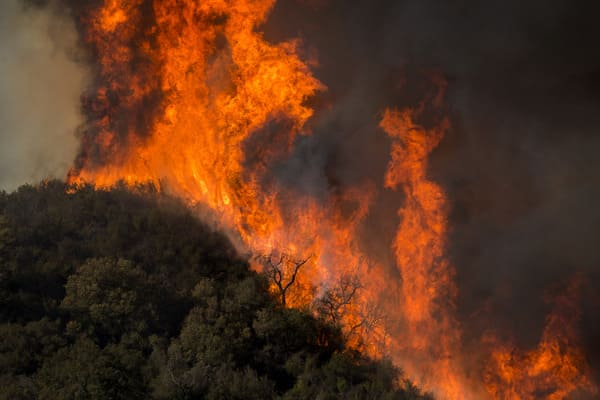
\includegraphics[width=0.5\linewidth]{pictures/intro.jpg}
        \caption{Feu de forêt à Malibu\footnote{National Geographic Education}}
        \label{fig:enter-label}
    \end{figure}
\end{frame}


\section{Un premier modèle de feux de forêt}
\section{Modèle d'Alexandridis pour les feux de forêt}
\section{Étude des transformations réalisables}

\begin{frame}{Sommaire \hyperlink{jump}{\beamerbutton{ }} \hypertarget{2}{\beamerbutton{ }}}
    \tableofcontents
\end{frame}

\begin{frame}{Un premier modèle de feux de forêt \hyperlink{jump}{\beamerbutton{ }} \hypertarget{3}{\beamerbutton{ }}}
    \begin{block}{Automate cellulaire (2D)}
        \begin{itemize}
            \item Une grille
            \item Un état par case
            \item Un ensemble de règles de transitions entre les états
        \end{itemize}
    \end{block}

    \visible<2-2>{\begin{figure}
        \centering
        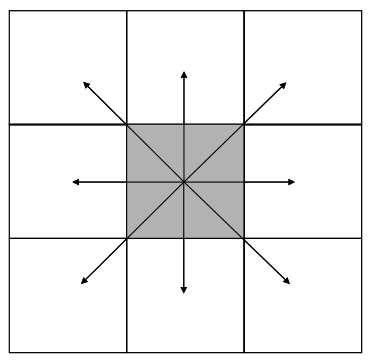
\includegraphics[width=0.25\linewidth]{pictures/moore.png}
        \caption{Voisinage de Moore \visible<2-2>{\footnote{Science Direct}}}
        \label{fig:enter-label}
    \end{figure}}
\end{frame}

\begin{frame}{Un premier modèle de feux de forêt \hyperlink{jump}{\beamerbutton{ }} \hypertarget{4}{\beamerbutton{ }}}
    \begin{block}{Types de cases :}
        \begin{itemize}
            \item Arbres
            \item Champs
            \item Feu
            \item Case brulée *
            \item Eau *
        \end{itemize}

        * Ne peuvent pas/plus bruler
    \end{block}

    \begin{figure}
        \begin{center}
            \renewcommand{\arraystretch}{2}
            \setlength{\extrarowheight}{-3pt}
            \begin{table}
                \begin{tabular}{ |C{2cm}|L{3cm}|C{3cm}|N }
                \hline
                $p_{b}$ & Voisin direct & Voisin diagonal \\
                \hline 
                Arbres & \centering $\tfrac{1}{8}$ & $\tfrac{1}{16}$ \\ 
                \hline
                Champs & \centering $\tfrac{1}{8}$ & $\tfrac{1}{16}$ \\
                \hline 
                \end{tabular}
            \end{table}
        \end{center}
        \caption{Changement d'états}
    \end{figure}
\end{frame}

\begin{frame}{Un premier modèle de feux de forêt \hyperlink{jump}{\beamerbutton{ }} \hypertarget{5}{\beamerbutton{ }}}
    \begin{figure}[!htb]
        \begin{minipage}{0.48\textwidth}
          \centering
          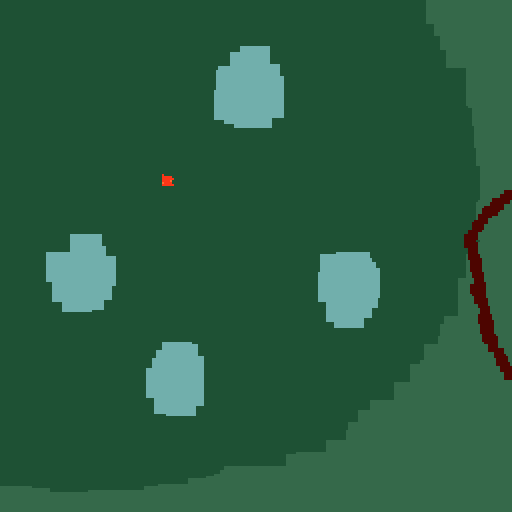
\includegraphics[width=.8\linewidth]{pictures/model1/land_before.png}
          \caption{À $t=0$}\label{Fig:Data1}
        \end{minipage}\hfill
        \begin{minipage}{0.48\textwidth}
          \centering
          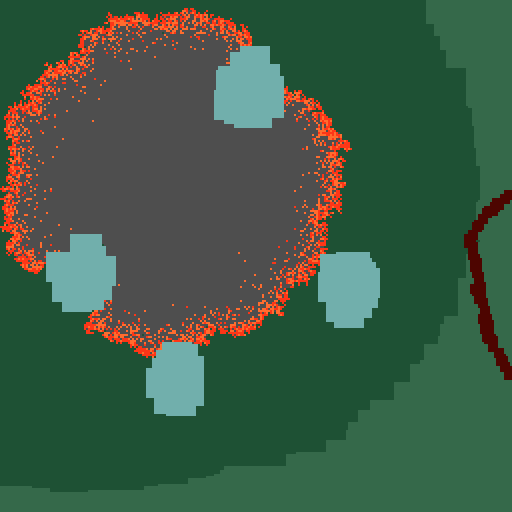
\includegraphics[width=.8\linewidth]{pictures/model1/land_200.png}
          \caption{À $t=200$}\label{Fig:Data2}
        \end{minipage}
     \end{figure}
\end{frame}

\begin{frame}{Vers le modèle d'Alexandridis \hyperlink{jump}{\beamerbutton{ }} \hypertarget{6}{\beamerbutton{ }}}
    \begin{block}{Idée}
        Il serait intéressant de prendre en compte des données du milieu : vent, densité de végétation
    \end{block}
\end{frame}

\begin{frame}{Modèle d'Alexandridis pour les feux de forêt \hyperlink{jump}{\beamerbutton{ }} \hypertarget{7}{\beamerbutton{ }}}
    \begin{block}{Nouveau type de case :}
        \begin{itemize}
            \item Arbres denses
        \end{itemize}
    \end{block}

    \hspace{1cm}

    \begin{block}{Règles de transition}
        Pour tout $(i,j,t) \in \mathbb{N}^3$, on a :
        \begin{itemize}
            \item Si $etat(i, j, t) = feu$, alors $etat(i, j, t+1) = brule$
            \item Si $etat(i, j, t) = feu$, alors $etat(i \pm 1, j \pm 1, t+1) = brule$ avec une probabilité $p_b$
            \item Si $etat(i, j, t) = brule$, alors $etat(i, j, t+1) = brule$
        \end{itemize}
    \end{block}
\end{frame}

\begin{frame}{Modèle d'Alexandridis pour les feux de forêt \hyperlink{jump}{\beamerbutton{ }} \hypertarget{8}{\beamerbutton{ }}}
    \begin{block}{Probabilité d'inflammage $p_b$}
        On a $p_b = p_h (1 + p_{veg}) (1 + p_{den}) p_{vent}$ avec $p_h = 0.27$ une constante
    \end{block}
    
    \begin{block}{Probabilité liée au vent $p_{vent}$}
        On a $p_{vent} = exp(0.045 \times v) \times exp (v \times 0.131 \times (cos(\theta) - 1))$ avec $\theta$ l'angle entre la propagation du feu et la direction du vent et $v$ la vitesse du vent (en $m/s$)
    \end{block}

    \begin{figure}
        \begin{center}
            \renewcommand{\arraystretch}{2}
            \setlength{\extrarowheight}{-3pt}
            \begin{table}
                \begin{tabular}{ |C{4cm}|L{2cm}|C{2cm}|N }
                \hline
                 & \centering $p_{veg}$ & $p_{den}$ \\
                \hline 
                Arbres & \centering $0.3$ & $0.3$ \\ 
                \hline
                Arbres denses & \centering $0.3$ & $0$ \\ 
                \hline
                Champs & \centering $-0.1$ & $0$ \\
                \hline 
                \end{tabular}
            \end{table}
        \end{center}
        \caption{Probabilités $p_{veg}$ et $p_{den}$ selon le type de végétation}
    \end{figure}
\end{frame}

\begin{frame}{Modèle d'Alexandridis pour les feux de forêt \hyperlink{jump}{\beamerbutton{ }} \hypertarget{9}{\beamerbutton{ }}}
    // TODO : Résultats sans vent sur la même grille et comparaison

    \begin{figure}[!htb]
        \begin{minipage}{0.48\textwidth}
          \centering
          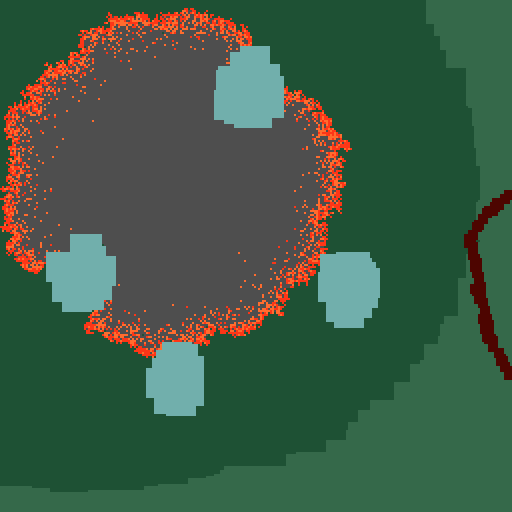
\includegraphics[width=.8\linewidth]{pictures/model1/land_200.png}
          \caption{Modèle 1 ($t=200$)}\label{Fig:Data1}
        \end{minipage}\hfill
        \begin{minipage}{0.48\textwidth}
          \centering
          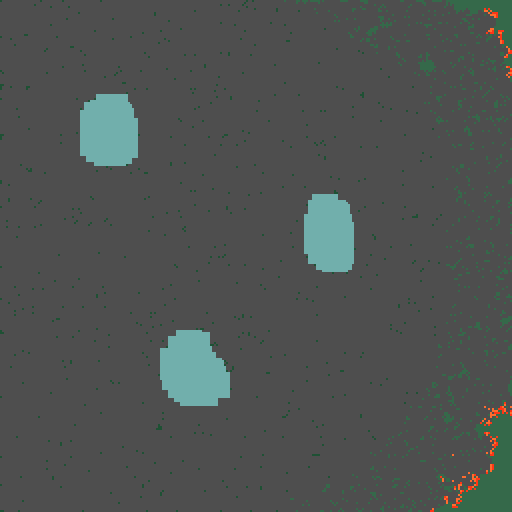
\includegraphics[width=.8\linewidth]{pictures/model2/land_200_nowind.png}
          \caption{Modèle 2 ($t=200$)}\label{Fig:Data2}
        \end{minipage}
     \end{figure}
\end{frame}

\begin{frame}{Modèle d'Alexandridis pour les feux de forêt \hyperlink{jump}{\beamerbutton{ }} \hypertarget{10}{\beamerbutton{ }}}
    // TODO : Prise en compte du vent dans une grille dense, et dans une grille pas dense

    // Vent : 15m/s

    \begin{figure}[!htb]
        \begin{minipage}{0.48\textwidth}
          \centering
          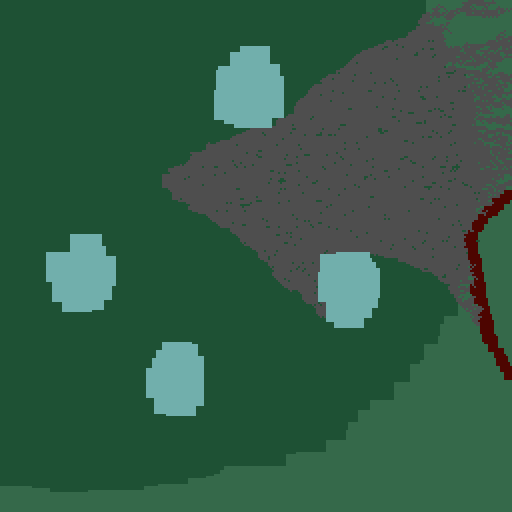
\includegraphics[width=.8\linewidth]{pictures/model2/land_200_wind_notdense.png}
          \caption{Vent à $15m/s$ vers l'est non dense ($t=200$)}\label{Fig:Data1}
        \end{minipage}\hfill
        \begin{minipage}{0.48\textwidth}
          \centering
          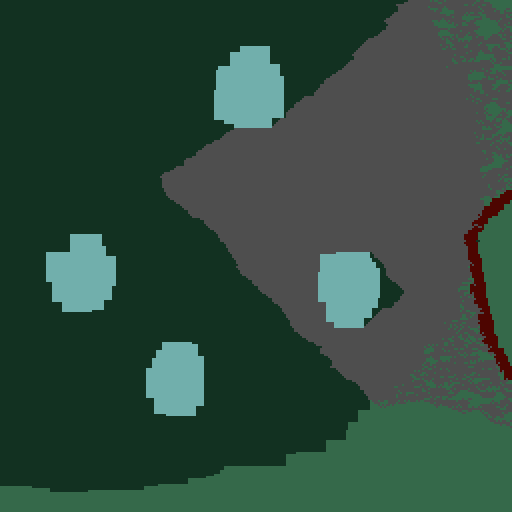
\includegraphics[width=.8\linewidth]{pictures/model2/land_200_wind_dense.png}
          \caption{Vent à $15m/s$ vers l'est dense ($t=200$)}\label{Fig:Data2}
        \end{minipage}
     \end{figure}
\end{frame}

\begin{frame}
    \frametitle{Navigateur \hypertarget{jump}{\beamerbutton{ }}}

    \hyperlink{1}{\beamerbutton{Diapo 1}} \\
    \hyperlink{2}{\beamerbutton{Diapo 2}}
\end{frame}

% \begin{frame}[
% t, % align text from top
% allowframebreaks, % allow brake frames
% fragile % allow verb content
% ]{main.c}
%     \scriptsize
%     \inputminted[breaklines,breakanywhere,fontsize=\tiny,
%     tabsize=2]{c}{code/main.c}
% \end{frame}
% \begin{frame}[
% t, % align text from top
% allowframebreaks, % allow brake frames
% fragile % allow verb content
% ]{misc.c}
%     \scriptsize
%     \inputminted[breaklines,breakanywhere,fontsize=\tiny,
%     tabsize=2]{c}{code/misc.c}
% \end{frame}
% \begin{frame}[
% t, % align text from top
% allowframebreaks, % allow brake frames
% fragile % allow verb content
% ]{grid.c}
%     \scriptsize
%     \inputminted[breaklines,breakanywhere,fontsize=\tiny,
%     tabsize=2]{c}{code/grid.c}
% \end{frame}
% \begin{frame}[
% t, % align text from top
% allowframebreaks, % allow brake frames
% fragile % allow verb content
% ]{typings.c}
%     \scriptsize
%     \inputminted[breaklines,breakanywhere,fontsize=\tiny,
%     tabsize=2]{c}{code/typings.c}
% \end{frame}
% \begin{frame}[
% t, % align text from top
% allowframebreaks, % allow brake frames
% fragile % allow verb content
% ]{draw.c}
%     \scriptsize
%     \inputminted[breaklines,breakanywhere,fontsize=\tiny,
%     tabsize=2]{c}{code/draw.c}
% \end{frame}

\end{document}
